\documentclass{beamer}
% Choose your desired theme
% \usetheme{Boadilla}
\usepackage[style=numeric]{biblatex}
\usepackage{listings}

\addbibresource{./cabi.bib}
\title{Pedaling Towards Progress}
\subtitle{Analyzing Washington, DC's Bikesharing system using Open-source tools}
\author{Maxwell Lindsay}
\institute{Van Oord}
\date{\today}

\begin{document}

\begin{frame}
    \titlepage
\end{frame}
\section{Introduction}
\begin{frame}
    % consider splitting into a few slides with more pictures
    \frametitle{Introduction to CaBi}
    \begin{columns}
        \column{0.5\textwidth}
        \begin{figure}
            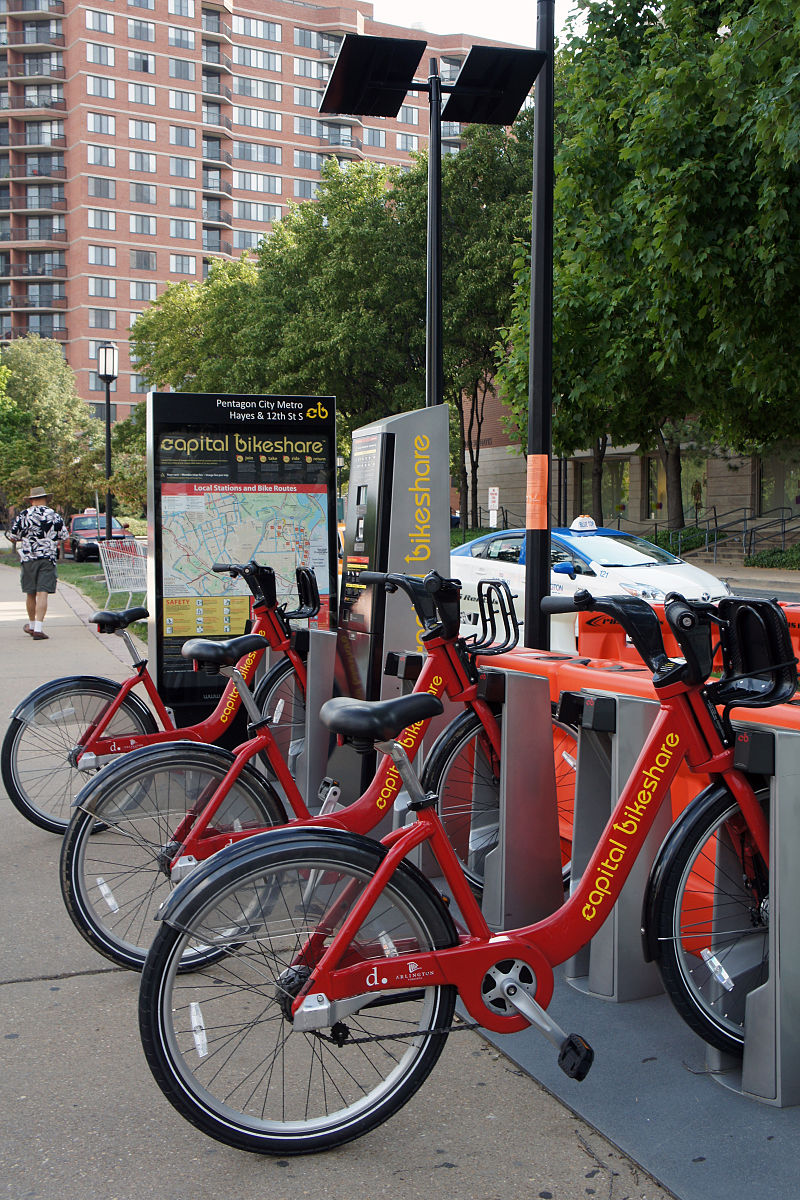
\includegraphics[]{800px-VA_07_2012_Capital_Bikeshare_4152.JPG}
            % \caption{By Mariordo (Mario Roberto Durán Ortiz) - Own work, CC BY-SA 3.0, https://commons.wikimedia.org/w/index.php?curid=20462784}
        \end{figure}
        \column{0.5\textwidth}
        \begin{itemize}
            \item Memberships are available for \$95 a year for unlimited trips under 45 minutes \cite{cabisite}. Casual users can pay \$1 to unlock the bike, then \$0.05 per minute.
            \item Primarily intended for short trips
            \item Docked bikeshare
            \item 700+ docks, ~35 million trips (so far)
        \end{itemize}

    \end{columns}
    \small{* recently, non-docked E-bikes that have been introduced}
\end{frame}

\begin{frame}
    \frametitle{The data}

    Capital Bikeshare publishes the following data about each trip on a monthly basis:

    \begin{itemize}
        \item start time
        \item end time
        \item start station index
        \item end station index
        \item Membership status of the rider (Member or Non-member?)
    \end{itemize}

    These data are available as csv files per month or year from Capital Bikeshare at https://ride.capitalbikeshare.com/system-data
\end{frame}

\begin{frame}
    \frametitle{My goal}

    \begin{itemize}
        \item Analyze all trips up to the present day
        \item Street-level estimates of bikeshare use
        \item Inspired by A blog post from Daniel J patterson from 2020
    \end{itemize}

\end{frame}

\section{Methodology}
\begin{frame}
    \frametitle{Overview of my approach}
    \begin{enumerate}
        \item Download CSVs of every trip
        \item Parse and normalize the CSVs using Pandas
        \item Find The number of trips between unique pairs of stations
        \item Build Valhalla routing tiles 
        \item Find a route between each station pair using Valhalla
        \item Aggregate the trip statistics across every single route
    \end{enumerate}
\end{frame}

\begin{frame}
    \frametitle{Download CSVs of every trip}


\end{frame}

\begin{frame}
    \frametitle{Parse and normalize the CSVs using Pandas}
    % sankey diagram?
    
\begin{itemize}
    \item Longer than a 4 hours
    
    This is an arbitrary threshold. However, the CaBi system is primarily intended for short trips, and the pricing reflects this. The bikes can be used for leisure and tourism, but they are priced to encourage users to change bikes regularly. Also, for the purposes of this project, long trips are less likely to have

    \item Starting and ending at the same station
    
    For obvious reasons, cannot easily be routed

    \item Stations with an invalid start or end station

    A number of trips in the dataset are missing a value for the start or ending point
\end{itemize}
    
\end{frame}

\begin{frame}
    \frametitle{Find unique trips between two stations}

\end{frame}

\begin{frame}
    \frametitle{Building a Valhalla Routing network}

    \begin{itemize}
        \item Download OSM tiles
        \item Build Valhalla routing network
        \item Use Pandas the start and end point of every unique trip
    \end{itemize}
\end{frame}

\begin{frame}
    \frametitle{Build PostGIS topology at the same time}
    \begin{itemize}
        \item Using PLpgSQL triggers, add a corresponding entry to the topogeometry table for every new entry to the routes tables
    \end{itemize}
\end{frame}

\begin{frame}
    \frametitle{Sum up the trips on every topological element}


    \begin{itemize}
        \item Using an SQL query, we can sum the trips on every unique street
    \end{itemize}

\end{frame}

\section{Conclusions}
\begin{frame}
    \frametitle{Lessons learned}

    \begin{itemize}
        \item Routing is *much* faster if you run it locally as binaries rather than a web api from a container
        \item Valhalla allows a like of parameters for bike routing and is lightning fast
    \end{itemize}



\end{frame}
\section{notes and thanks}
\begin{frame}
    \frametitle{Shoutouts}

    \begin{itemize}
        \item GIS-OPS for their thoughtful and intuitive Valhalla Docker containers
        \item
    \end{itemize}



\end{frame}
\end{document}
